\documentclass{standalone}
\usepackage{graphicx}	
\usepackage{amssymb, amsmath}
\usepackage{color}

\usepackage{tikz}
\usetikzlibrary{intersections, backgrounds, math}
\usepackage{pgfmath}

\definecolor{light}{RGB}{220, 188, 188}
\definecolor{mid}{RGB}{185, 124, 124}
\definecolor{dark}{RGB}{143, 39, 39}
\definecolor{highlight}{RGB}{180, 31, 180}
\definecolor{light_teal}{RGB}{107, 142, 142}
\definecolor{mid_teal}{RGB}{72, 117, 117}
\definecolor{dark_teal}{RGB}{29, 79, 79}
\definecolor{gray10}{gray}{0.1}
\definecolor{gray20}{gray}{0.2}
\definecolor{gray30}{gray}{0.3}
\definecolor{gray40}{gray}{0.4}
\definecolor{gray60}{gray}{0.6}
\definecolor{gray70}{gray}{0.7}
\definecolor{gray80}{gray}{0.8}
\definecolor{gray90}{gray}{0.9}
\definecolor{gray95}{gray}{0.95}

\begin{document}

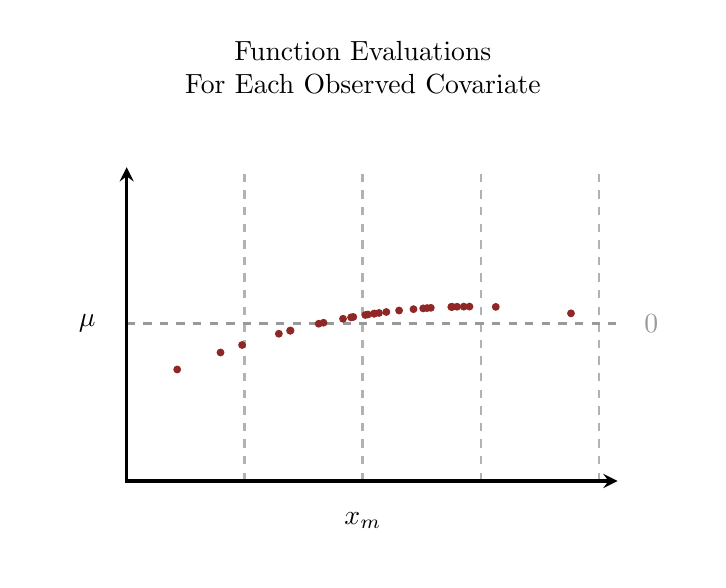
\begin{tikzpicture}[scale=1.0]

  \begin{scope}[shift={(8.5, 0)}]
    \draw[white] (-4.25, -3) rectangle (4.25, 3.75);
    
    \node[align=center] at (0, 3.25) { Function Evaluations\\For Each Observed Covariate };
    
    \foreach \b in {-3.0, -1.5,  0.0,  1.5,  3.0} {
      \draw[gray70, dashed, line width=1] (\b, -2) -- (\b, 2);
    }
    
    \draw[gray60, dashed, line width=1] (-3, 0) -- (3.25, 0);   
    \node[gray60, anchor=west] at (3.1, 0)  { $\quad 0$ };
    
    \foreach \x/\mu in {0.205/0.134, 0.863/0.199, -0.150/0.078, 0.142/0.125, 0.147/0.126, 
                        1.354/0.215, -0.919/-0.090, -0.561/-0.003, 0.298/0.146, 1.134/0.211, 
                        -0.924/-0.091, 0.064/0.114, -0.500/0.010, 1.196/0.213, -0.122/0.083, 
                        -2.358/-0.584, -0.252/0.060, 2.643/0.129, 1.281/0.214, -1.808/-0.368, 
                        -1.067/-0.130, 1.688/0.211, 0.766/0.192, 0.643/0.182, 0.031/0.108, 
                        0.815/0.196, 0.460/0.165, -1.534/-0.273, 1.126/0.211, 1.124/0.211} {
       \fill[dark] (\x, \mu) circle(0.05);
    }
     
    \draw [->, >=stealth, line width=1.25] (-3.00, -2.015) -- +(0, 4);
    \draw [->, >=stealth, line width=1.25] (-3.015, -2.00) -- +(6.25, 0);
    
    \node at (-3.5, 0) { $\mu$ };
    \node at (0, -2.5) { $x_{m}$ };
  \end{scope}
    
\end{tikzpicture}

\end{document}  